\documentclass[10pt,letterpaper,bibliography=totocnumbered]{scrartcl}

\usepackage[letterpaper,margin=1.2in]{geometry}
\usepackage{helvet}
\usepackage{graphicx}
\usepackage[hyphens]{url}
\usepackage{hyperref}
\usepackage[all]{hypcap} 
\usepackage{xcolor}
\usepackage{listings}
\usepackage[T1]{fontenc}
\usepackage{verbatim}

\lstset{
    basicstyle=\scriptsize,
    numbers=left,
    numberstyle=\scriptsize,
    stepnumber=1,
    numbersep=5pt,
    showspaces=false,
    showstringspaces=false,
    showtabs=false,
    frame=shadowbox,
    tabsize=4,
    captionpos=b,
    breaklines=true,
    breakatwhitespace=false,
    keywordstyle=\color{blue!70},
    commentstyle=\color{red!50!green!50!blue!50},
    rulesepcolor=\color{red!20!green!20!blue!20},
    numberbychapter=false,
    stringstyle=\ttfamily
}

\setcounter{tocdepth}{2}

\hypersetup{colorlinks=true,
breaklinks=true,
urlcolor=blue,
linkcolor=black
}

\begin{document}

\author{Mathew Chaney}
\title{Assignment 8}
\subtitle{Fall 2014\\ CS595 Web Science\\ Dr. Michael Nelson}
\maketitle
\newpage

\tableofcontents
% \listoffigures
\lstlistoflistings

\section{Question 1}

\subsection{Question}
\verbatiminput{q1/q1.txt}

\subsection{Answer}
Using Dr. Michael Nelson's Twitter account and the Twitter API \cite{api:twitter}, specifically the GET friends/list \cite{api:twitter_friendslist} request, all of Dr. Nelson's Twitter friends were obtained and saved to the file called {\tt friends}. This method also uses the API's paginating scheme: when there are a large number of results for a query, the API will send a cursor index to show that there are more results to process and that more requests are needed. The code to do this is in Listing \ref{listing:get_friends}. 

% \lstinputlisting[language=Python, caption={Getting the friends list}, label=listing:get_friends,linerange={38-57},firstnumber=38]{q1/get_friends.py}

\clearpage

To reduce the impact of high HTTP traffic, the Twitter API rate-limits most requests -- the one needed to obtain a user's friends list has a limit of fifteen message per fifteen minutes. Any requests received from a user or service that has reached the limit will be denied. To ensure no HTTP requests are sent after the limit has been reached the script will sleep until the limit resets. This is accomplished using Python's {\tt time} package \cite{py:time} and the methods shown in Listing \ref{listing:wait}.

% \lstinputlisting[language=Python, caption={Waiting for API request limit reset}, label=listing:wait,linerange={24-36},firstnumber=24]{q1/get_friends.py}

The {\tt get\_limit} method uses the API to find the number of available requests remaining for the GET friends/list method and also the time at which the limit will reset, received as seconds since the Unix epoch \cite{misc:stack_unixepoch}. This method, combined with the {\tt wait\_for\_reset} method, allowed the script to restart after an interruption and only require waiting for the appropriate amount of time. The sleep time was extended by 5 seconds to allow for a small buffer in case of mathematical errors.\\

The friends of Dr. Nelson's friends were then obtained with the same {\tt get\_friends} method from Listing \ref{listing:get_friends} and stored in a file called {\tt friend\_counts}, each on a single line preceeded by their friend count. All of these operations were controlled by a main method, which is shown in Listing \ref{listing:main}.

% \lstinputlisting[language=Python,caption={Main method}, label=listing:main, linerange={59-82},firstnumber=59]{q1/get_friends.py}

\clearpage

The {\tt friend\_counts} file was ordered in place with the Unix command in Listing \ref{listing:sort}. 

\begin{lstlisting}[language=Bash,caption={Sort command},label=listing:sort]
[mchaney@mchaney-l a5]$ cat friend_counts | sort -g -o friend_counts
\end{lstlisting}

This file was then processed by the R script shown in Listing \ref{listing:graph} to produce the graph in Figure \ref{fig:friend_graph}

% \lstinputlisting[language=R, caption={Graph Creation Script}, label=listing:graph]{q1/plot_friends.R}

\clearpage
The median, mean and standard deviation were all calculated, with the median, mean and median plus one standard deviation plotted as horizontal lines that intersect the data plot at their y-values. Only a single line was drawn for the standard deviation because the lower-end value was negative, and thus off the graph. 

% \begin{figure}[h!]
% \centering
% \fbox{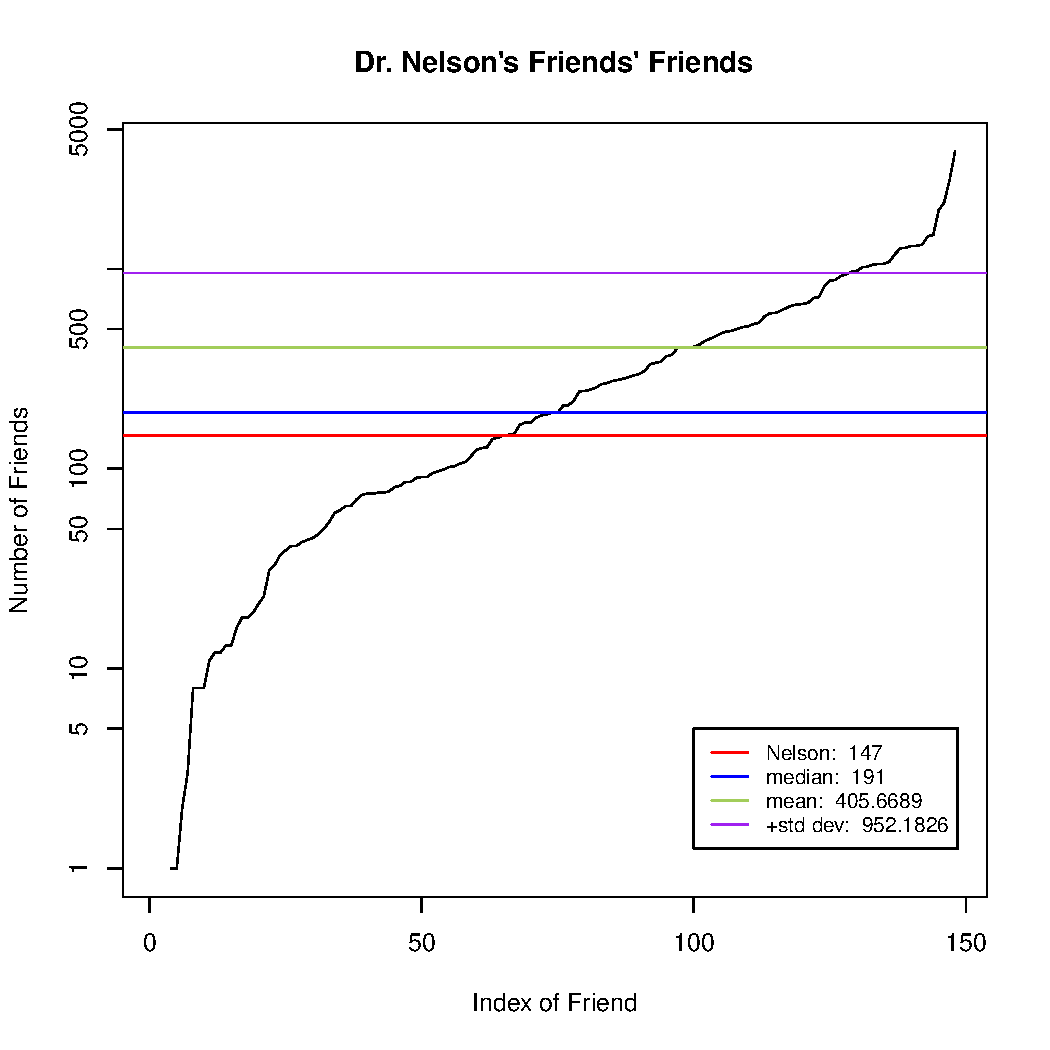
\includegraphics[scale=0.75]{q1/friend_plot.pdf}}
% \caption{The Friendship Graph}
% \label{fig:friend_graph}
% \end{figure}

\bibliography{report}
\bibliographystyle{unsrt}

\end{document}
